\documentclass[10pt]{beamer}

\usetheme{Oxygen}
\usepackage{hyperref}
\usepackage[compatibility=false]{caption}
\usepackage{thumbpdf}
\usepackage{wasysym}
\usepackage{ucs}
\usepackage[utf8]{inputenc}
\usepackage{pgf,pgfarrows,pgfnodes,pgfautomata,pgfheaps,pgfshade}
\usepackage{verbatim}
\usepackage{listing}
\usepackage{url}
\usepackage{cite}
\usepackage{minted}

\pdfinfo
{
  /Title       (iOS Application Development)
  /Creator     (TeX)
  /Author      (Chris Zelenak)
}


\title{iOS Application Development}
\subtitle{Day 3}
\author{Chris Zelenak}
\date{06/24/2010}

\begin{document}



\frame{\titlepage}

\section*{}
\begin{frame}
  \frametitle{Outline}
  \tableofcontents[section=1,hidesubsections]
\end{frame}

\AtBeginSection[]
{
  \frame<handout:0>
  {
    \frametitle{Outline}
    \tableofcontents[currentsection,hideallsubsections]
  }
}

\AtBeginSubsection[]
{
  \frame<handout:0>
  {
    \frametitle{Outline}
    \tableofcontents[sectionstyle=show/hide,subsectionstyle=show/shaded/hide]
  }
}

\newcommand<>{\highlighton}[1]{%
  \alt#2{\structure{#1}}{{#1}}
}

\newcommand{\icon}[1]{\pgfimage[height=1em]{#1}}

 

  
    
% BEGIN SECTION Core Data and SQLite
\section{Core Data and SQLite}
\begin{frame}[fragile]
  \frametitle{Core Data and SQLite}
  1. Core Data and SQLite
\end{frame}


    
\begin{frame}[fragile]
  \frametitle{NSManagedObject and beyond}
  NSManagedObject is the primary element of working with your core data store. It represents a single entity's worth of information in the database that backs your app. The actual data for the entity is able to be queried via the valueForKey and setValue:forKey: methods of NSManagedObject.

\end{frame}

\begin{frame}[fragile]
  \frametitle{NSManagedObject and beyond}
  NSManagedObject changes are queued to an NSManagedObjectContext which is roughly equivalent to a database transaction; it provides locking, commit/rollback and undo/redo functionality for object changes.

\end{frame}

\begin{frame}[fragile]
  \frametitle{NSManagedObject and beyond}
  NSEntityDescription describes the schema associated with a specific type of NSManagedObject; a database table is similar in the way that it describes the layout of its child rows.

\end{frame}

\begin{frame}[fragile]
  \frametitle{NSManagedObject and beyond}
  NSManagedObjectModels are created by the programmer, and are collections of NSEntityDescriptions.

\end{frame}

\begin{frame}[fragile]
  \frametitle{NSManagedObject and beyond}
  NSPersistentStore represents the actual physical location of your Core Data objects, and can be a database, an XML file, or any other other physical manifestation of data for which an NSPersistentStore has been written.

\end{frame}

\begin{frame}[fragile]
  \frametitle{NSManagedObject and beyond}
  You can create your own NSManagedObjectModel subclasses that provide convenient abstractions over NSManagedObjectModel.

\end{frame}

\begin{frame}[fragile]
  \frametitle{NSManagedObject and beyond}
  To get an instance of an NSManagedObject that is able to be saved to the NSPersistentStore, use:
\begin{listing}[H]
    \begin{minted}[resetmargins=true,fontsize=\footnotesize]{objectivec}
  
  NSManagedObject * newObject = [NSEntityDescription
                                 insertNewObjectForEntityForName:@"EntityName"
                                 inManagedObjectContext:managedObjectContext];
                
  \end{minted}
    \caption{Getting a new NSManagedObject that will eventually be saved to an NSPersistentStore}
    \label{listing:39}
  \end{listing}

\end{frame}

\begin{frame}[fragile]
  \frametitle{NSManagedObject and beyond}
  To save changes to all current NSManagedObjects currently managed by an NSManagedObjectContext:
\begin{listing}[H]
    \begin{minted}[resetmargins=true,fontsize=\footnotesize]{objectivec}
  
  NSError * error = nil;
  [managedObjectContext save:&error];
  if(error){
      NSLog(@"Couldn't save objects, %@", error);
  } 
                
  \end{minted}
    \caption{Saving changed objects}
    \label{listing:40}
  \end{listing}

\end{frame}

    
\begin{frame}[fragile]
  \frametitle{NSPredicate and NSFetchRequest}
  Actually fetching objects from the Core Data store requires you to build queries using NSPredicate or NSFetchRequest.

\end{frame}

\begin{frame}[fragile]
  \frametitle{NSPredicate and NSFetchRequest}
  The syntax for NSPredicate and NSFetchRequest requests is similar to SQL, but not identical.

\end{frame}

\begin{frame}[fragile]
  \frametitle{NSPredicate and NSFetchRequest}
  \begin{listing}[H]
    \begin{minted}[resetmargins=true,fontsize=\footnotesize]{objectivec}
  
  NSPredicate * searchPredicate = [NSPredicate
                           predicateWithFormat:@"(firstName = 'Chris') AND "
                                        @"(lastName BEGINSWITH 'Zel') AND "
                                        @"(age BETWEEN {%i,%i})", 20, 30];
                
  \end{minted}
    \caption{NSPredicate example}
    \label{listing:41}
  \end{listing}
\begin{block}{See more..}
  
  Read more about writing NSPredicates in the "Predicate Programming Guide" in
  the XCode documentation.
                
  \end{block}

\end{frame}

\begin{frame}[fragile]
  \frametitle{NSPredicate and NSFetchRequest}
  You can also build named NSFetchRequests in the .xcdmodel for your entities. \begin{figure}[htb]
  \begin{center}
  
  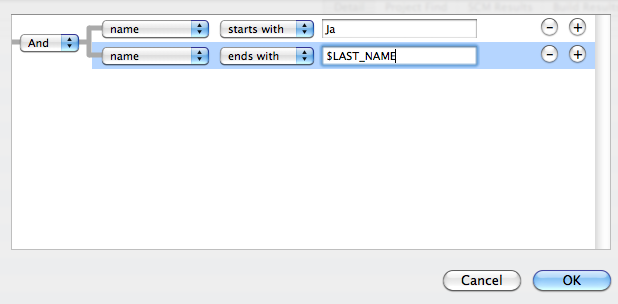
\includegraphics[scale=0.5]{PredicateBuilder.png}
                
  \caption{Predicate builder}
  \end{center}
  \end{figure}

\end{frame}

\begin{frame}[fragile]
  \frametitle{NSPredicate and NSFetchRequest}
  \begin{listing}[H]
    \begin{minted}[resetmargins=true,fontsize=\footnotesize]{objectivec}
  
  NSFetchRequest * req = [managedObjectModel
                           fetchRequestFromTemplateWithName:@"requestByName"
                           substitutionVariables:[NSDictionary
                              dictionaryWithObjectsAndKeys:
                                @"Pwnsberry", @"LAST_NAME", nil]];
                
  \end{minted}
    \caption{Stored NSPredicate example}
    \label{listing:42}
  \end{listing}

\end{frame}

    
\begin{frame}[fragile]
  \frametitle{Lab 6}
  Create a property list with the names of the students in the class

\end{frame}

\begin{frame}[fragile]
  \frametitle{Lab 6}
  Create the xcdmodel that describes the entities

\end{frame}

\begin{frame}[fragile]
  \frametitle{Lab 6}
  Initialize the Core Data persistence layer

\end{frame}

\begin{frame}[fragile]
  \frametitle{Lab 6}
  Use NSUserDefaults to detect whether or not the app has been started before

\end{frame}

\begin{frame}[fragile]
  \frametitle{Lab 6}
  Perform the import if the app has never been started before

\end{frame}

\begin{frame}[fragile]
  \frametitle{Lab 6}
  Pass the user and image data on to the details controller

\end{frame}

    

% END SECTION Core Data and SQLite
   
  

  
    
% BEGIN SECTION Networking ( NSURLRequest )
\section{Networking ( NSURLRequest )}
\begin{frame}[fragile]
  \frametitle{Networking ( NSURLRequest )}
  2. Networking ( NSURLRequest )
\end{frame}


    
\begin{frame}[fragile]
  \frametitle{NSURL, NSURLRequest,  NSMutableURLRequest AND NSURLConnection}
  NSURL is meant to only represent a single resource location

\end{frame}

\begin{frame}[fragile]
  \frametitle{NSURL, NSURLRequest,  NSMutableURLRequest AND NSURLConnection}
  NSURL can be allocated to represent either a filesystem location, or a web resource

\end{frame}

\begin{frame}[fragile]
  \frametitle{NSURL, NSURLRequest,  NSMutableURLRequest AND NSURLConnection}
  NSURLRequest and NSMutableURLRequest represent specific web resources that you'd like to initiate a connection to; NSURLRequest should be used for simple GET HTTP requests, while NSMutableURLRequests can be used for more complex HTTP requests.

\end{frame}

\begin{frame}[fragile]
  \frametitle{NSURL, NSURLRequest,  NSMutableURLRequest AND NSURLConnection}
  NSMutableURLRequest allows you to set HTTP headers, the HTTP method used, and the request body.

\end{frame}

\begin{frame}[fragile]
  \frametitle{NSURL, NSURLRequest,  NSMutableURLRequest AND NSURLConnection}
  NSURLRequest and NSMutableURLRequest both by default only work with HTTP requests

\end{frame}

\begin{frame}[fragile]
  \frametitle{NSURL, NSURLRequest,  NSMutableURLRequest AND NSURLConnection}
  NSURLConnection initiates the download and returns the NSHTTPURLResponse which contains the body of the response, as well as http status code and response headers.

\end{frame}

\begin{frame}[fragile]
  \frametitle{NSURL, NSURLRequest,  NSMutableURLRequest AND NSURLConnection}
  NSURLConnection can send data both synchronously or asynchronously; the response information is passed back to the connection delegate via the informal NSURLConnection delegate.

\end{frame}

    
\begin{frame}[fragile]
  \frametitle{Networking Lab}
  Create a new UIVIewController

\end{frame}

\begin{frame}[fragile]
  \frametitle{Networking Lab}
  Add an NSURLConnection object

\end{frame}

\begin{frame}[fragile]
  \frametitle{Networking Lab}
  Download the plist object and deserialize it

\end{frame}

\begin{frame}[fragile]
  \frametitle{Networking Lab}
  Load the tableView with the new data

\end{frame}

    
\begin{frame}[fragile]
  \frametitle{( ASIHttpRequest, EasyURLDownloader )}
  ASIHttpRequest gives you a full-featured HTTP library enhancement; cookie persistence support, enhanced HTTP auth support, S3 support and more. \url{http://github.com/pokeb/asi-http-request/}

\end{frame}

\begin{frame}[fragile]
  \frametitle{( ASIHttpRequest, EasyURLDownloader )}
  EasyURLDownloader gives you a simple library to perform asynchronous GET downloads in the background \url{http://github.com/netshade/EasyUrlDownloader}

\end{frame}

    
\begin{frame}[fragile]
  \frametitle{SOAP and REST Webservices}
  You can roll your own webservice access, but you don't have ot.

\end{frame}

\begin{frame}[fragile]
  \frametitle{SOAP and REST Webservices}
  ObjectiveResource makes accessing REST services with ObjectiveC incredibly easy.

\end{frame}

\begin{frame}[fragile]
  \frametitle{SOAP and REST Webservices}
  WSMakeStubs will create stubs for you that shim out the available endpoints of a WSDL web service.

\end{frame}

\begin{frame}[fragile]
  \frametitle{SOAP and REST Webservices}
  ObjectiveResource is available at \url{http://github.com/yfactorial/objectiveresource}

\end{frame}

\begin{frame}[fragile]
  \frametitle{SOAP and REST Webservices}
  WSMakeStubs is a binary included with your SDK

\end{frame}

    

% END SECTION Networking ( NSURLRequest )
   
  

  
    
% BEGIN SECTION Getting your application on the device
\section{Getting your application on the device}
\begin{frame}[fragile]
  \frametitle{Getting your application on the device}
  3. Getting your application on the device
\end{frame}


    
\begin{frame}[fragile]
  \frametitle{Development certificates, Distribution certificates}
  Log in to the iPhone developer portal and request a developer certificate

\end{frame}

\begin{frame}[fragile]
  \frametitle{Development certificates, Distribution certificates}
  Explain Key requests

\end{frame}

\begin{frame}[fragile]
  \frametitle{Development certificates, Distribution certificates}
  Download and install certificate

\end{frame}

\begin{frame}[fragile]
  \frametitle{Development certificates, Distribution certificates}
  Create development provisioning profile with devices

\end{frame}

\begin{frame}[fragile]
  \frametitle{Development certificates, Distribution certificates}
  Assign development provisioning profile

\end{frame}

\begin{frame}[fragile]
  \frametitle{Development certificates, Distribution certificates}
  AdHoc and Store based distribution reserved for Agents only

\end{frame}

    

% END SECTION Getting your application on the device
   
  

  
    
% BEGIN SECTION Using Instruments
\section{Using Instruments}
\begin{frame}[fragile]
  \frametitle{Using Instruments}
  4. Using Instruments
\end{frame}


    
\begin{frame}[fragile]
  \frametitle{Always, always, always memory leak check}
  Opening up the Leaks tool and examining your application behavior

\end{frame}

\begin{frame}[fragile]
  \frametitle{Always, always, always memory leak check}
  Examining specific leaks

\end{frame}

\begin{frame}[fragile]
  \frametitle{Always, always, always memory leak check}
  Understanding the Leaks tool

\end{frame}

    
\begin{frame}[fragile]
  \frametitle{Always, always, always activity monitor check}
  Using Activity Monitor to monitor your current system state

\end{frame}

    

% END SECTION Using Instruments
   
  

  
    
% BEGIN SECTION Distributing your app to others
\section{Distributing your app to others}
\begin{frame}[fragile]
  \frametitle{Distributing your app to others}
  5. Distributing your app to others
\end{frame}


    
\begin{frame}[fragile]
  \frametitle{The process you need to know}
  Releasing your app to others in beta form

\end{frame}

\begin{frame}[fragile]
  \frametitle{The process you need to know}
  What is an .ipa file

\end{frame}

\begin{frame}[fragile]
  \frametitle{The process you need to know}
  How to send your .ipa file to others

\end{frame}

    
\begin{frame}[fragile]
  \frametitle{The URLs you need to know}
  \url{http://developer.apple.com/iphone/} is the frontend to most Apple web services

\end{frame}

\begin{frame}[fragile]
  \frametitle{The URLs you need to know}
  \url{http://itunesconnect.apple.com/} is the URL to access the app-release frontend and store management services provided by Apple

\end{frame}

    

% END SECTION Distributing your app to others
   
  

  
% BEGIN SECTION Questions
\section{Questions}
\begin{frame}[fragile]
  \frametitle{Questions}
  
\end{frame}

% END SECTION Questions

  


\bibliography{slides}{}
\bibliographystyle{plain}

\end{document}
